\documentclass[11pt,a4paper,oneside,openany,indonesian]{report}
\usepackage[a4paper,top=25mm,bottom=25mm,left=30mm,right=25mm,headheight=16pt,headsep=7mm,footskip=12mm]{geometry}
\usepackage{iftex}
\ifLuaTeX
  \usepackage[bidi=basic,shorthands=off,provide=*]{babel}
\else
  \usepackage[bidi=default,shorthands=off,provide=*]{babel}
\fi
\ifPDFTeX\else\babelfont{rm}[]{Charter}\fi
\usepackage{hyperref}
% Shared preamble for the Jakarta TGA chapters.
\usepackage{xcolor}
\usepackage{graphicx}
\usepackage{amsmath,amssymb}
\usepackage{iftex}
\ifPDFTeX
  \usepackage[T1]{fontenc}
  \usepackage[utf8]{inputenc}
  \usepackage{textcomp}
\else
  \usepackage{unicode-math}
  \defaultfontfeatures{Scale=MatchLowercase}
  \defaultfontfeatures[\rmfamily]{Ligatures=TeX,Scale=1}
\fi
\usepackage{lmodern}
\ifPDFTeX\else
  \setmainfont[]{Times New Roman}
  \setsansfont[]{Arial}
  \IfFontExistsTF{Consolas}{\setmonofont[]{Consolas}}{\setmonofont[]{Courier New}}
\fi
\IfFileExists{microtype.sty}{\usepackage{microtype}}{}
\usepackage{longtable,booktabs,array,tabularx,adjustbox,calc}
\usepackage{pdflscape}
\usepackage{caption}
\captionsetup[table]{skip=6pt}
\newcounter{none}
\usepackage{float}
\usepackage{setspace}
\usepackage{ragged2e}
\usepackage{titlesec}
\usepackage{enumitem}
\usepackage{needspace}
\usepackage{fancyhdr}
\usepackage{newunicodechar}
\usepackage{bookmark}
\usepackage{xurl}
\usepackage{csquotes}
\usepackage[backend=biber,style=authoryear,maxcitenames=2,maxbibnames=99,uniquelist=false,uniquename=false]{biblatex}
\DeclareLanguageMapping{indonesian}{english}
\DefineBibliographyStrings{english}{and={dan},andothers={dkk\adddot}}
\DefineBibliographyStrings{indonesian}{and={dan},andothers={dkk\adddot}}
\AtBeginDocument{\renewcommand*{\finalnamedelim}{\addspace dan\space}}
\addbibresource{references.bib}
\DeclareFieldFormat{title}{#1}
\DeclareFieldFormat[article,inbook,incollection,inproceedings,inreference,patent,thesis,unpublished]{title}{#1}
\AtBeginBibliography{\small\setlength{\bibitemsep}{0.15em}}

\newunicodechar{∅}{\ensuremath{\varnothing}}

% Placeholder untuk gambar yang dibuat manual (peta GIS). Ganti dengan \includegraphics setelah berkas target tersedia.
\newcommand{\GambarPlaceholder}[2][7cm]{%
  \fbox{\parbox[c][#1][c]{0.92\linewidth}{\centering\small
    \textbf{PLACEHOLDER GAMBAR}\\[0.6em]#2}}}

\definecolor{Ink}{HTML}{222222}
\definecolor{RuleGray}{HTML}{666666}

\AtBeginDocument{%
  \hypersetup{linkcolor=Ink,citecolor=Ink,urlcolor=Ink,pdfborder={0 0 0}}%
  \urlstyle{same}%
}

\setstretch{1.5}
\setlength{\parindent}{1.1em}
\setlength{\parskip}{0.28em}
\setlength{\emergencystretch}{2.5em}
\clubpenalty=10000
\widowpenalty=10000
\displaywidowpenalty=10000
\raggedbottom

\setlist[itemize]{leftmargin=1.7em,itemsep=0.25em,topsep=0.35em}
\setlist[enumerate]{leftmargin=1.9em,itemsep=0.25em,topsep=0.35em}

\titleformat{\chapter}[display]
  {\normalfont\bfseries\centering\color{Ink}}
  {}{0pt}{\Large\hyphenpenalty=10000\exhyphenpenalty=10000}
\titlespacing*{\chapter}{0pt}{-6pt}{18pt}
\titleformat{\section}{\Needspace{4\baselineskip}\large\bfseries\color{Ink}}{\thesection}{0.7em}{}
\titleformat{\subsection}{\Needspace{3\baselineskip}\normalsize\bfseries\color{Ink}}{\thesubsection}{0.7em}{}
\titleformat{\subsubsection}{\Needspace{3\baselineskip}\normalsize\bfseries\color{Ink}}{\thesubsubsection}{0.7em}{}

\pagestyle{plain}
\fancyhf{}
\fancyfoot[C]{\thepage}
\renewcommand{\headrulewidth}{0pt}
\renewcommand{\footrulewidth}{0pt}
\fancypagestyle{plain}{%
  \fancyhf{}
  \fancyfoot[C]{\thepage}
  \renewcommand{\headrulewidth}{0pt}
}

\renewcommand{\arraystretch}{1.2}
\setlength{\extrarowheight}{1pt}
\setlength{\tabcolsep}{4pt}
\providecommand{\tightlist}{\setlength{\itemsep}{0pt}\setlength{\parskip}{0pt}}
\setlength{\LTpre}{0.5em}
\setlength{\LTpost}{0.8em}
\AtBeginEnvironment{longtable}{\footnotesize\setstretch{1.0}\setlength{\tabcolsep}{3pt}\setlength{\extrarowheight}{1pt}}
\AtBeginEnvironment{table}{\setstretch{1.0}}
\AtBeginEnvironment{figure}{\setstretch{1.0}}
\AtBeginEnvironment{quote}{\small\setlength{\leftskip}{1.2em}\setlength{\rightskip}{1.2em}}


\hypersetup{
  pdftitle={Bab 2 Kajian Pustaka},
  pdfauthor={Mahastri Laksita Sam Widita},
  pdflang={id-ID},
  hidelinks
}

\title{\textbf{Borrowed Size atau Agglomeration Shadow?}\\[0.4em]
Analisis Hubungan Integrasi Metropolitan dengan Kematangan Pusat-Pusat Sekunder di Kawasan Aglomerasi Jakarta}
\providecommand{\subtitle}[1]{\gdef\thesubtitle{#1}}
\subtitle{Bab 2 Kajian Pustaka}
\author{Mahastri Laksita Sam Widita\\NIM 22/503065/TK/54947\\[0.5em]
Pembimbing: Rendy Bayu Aditya\\[0.5em]
Program Studi Perencanaan Wilayah dan Kota\\
Departemen Teknik Arsitektur dan Perencanaan\\
Fakultas Teknik\\
Universitas Gadjah Mada}
\date{Kabupaten Sleman, Daerah Istimewa Yogyakarta\\2026}

\makeatletter
\renewcommand{\maketitle}{%
  \begin{titlepage}
    \centering
    {\Large\bfseries TUGAS AKHIR\par}
    \vfill
    {\LARGE\bfseries \@title\par}
    \vspace{1.2cm}
    {\large \thesubtitle\par}
    \vfill
    {\large \@author\par}
    \vfill
    {\large \@date\par}
  \end{titlepage}}
\makeatother

\begin{document}
\maketitle
\tableofcontents
\clearpage
\setcounter{chapter}{1}
\chapter{Kajian Pustaka}

\section{Penjelasan konsep-konsep kunci}

Konsep dalam bab ini dipakai untuk membedakan objek yang sering tercampur dalam pembahasan metropolitan. Ukuran lokal, fungsi, kinerja, aksesibilitas, konektivitas, dan integrasi fungsional bukan sinonim. Sebuah pusat sekunder dapat mempunyai penduduk besar, akses yang baik, dan arus keluar yang kuat pada saat yang sama. Susunan seperti itu belum cukup untuk disebut peminjaman ukuran atau bayangan aglomerasi.

\subsection{Ekonomi aglomerasi dan disekonomi aglomerasi}

Ekonomi aglomerasi adalah manfaat yang muncul ketika rumah tangga dan perusahaan berdekatan dengan banyak orang, pekerja, pemasok, pengetahuan, infrastruktur, dan amenitas. Mekanisme yang sering digunakan untuk menjelaskannya ialah berbagi, mencocokkan, dan belajar: berbagi fasilitas atau input, mencocokkan kebutuhan perusahaan dengan tenaga kerja, serta memperoleh pembelajaran dan pengetahuan dari interaksi yang berulang \parencite{durantonpuga2004}. Konsentrasi juga menimbulkan biaya, seperti kemacetan, harga lahan, polusi, tekanan jaringan, dan kompetisi atas sumber daya. Karena manfaat dan biaya bergerak bersama dengan cara yang berbeda, aglomerasi tidak boleh diperlakukan sebagai keuntungan yang selalu positif.

Dalam penelitian ini, teori aglomerasi menjadi garis dasar untuk membaca hubungan ukuran dan fungsi. Jika pusat yang lebih besar cenderung menopang lebih banyak fungsi, maka fungsi pusat kecil yang melebihi ekspektasi ukurannya perlu dijelaskan melalui relasi lain, karakteristik khusus, atau kesalahan pengukuran. Kenaikan kepadatan juga tidak langsung berarti kenaikan produktivitas; arah hubungan dapat berubah menurut sektor, skala, kelompok sosial, dan kondisi wilayah.

\subsection{Ukuran lokal, fungsi metropolitan, dan kinerja}

Tiga objek dipisahkan sejak awal. Ukuran lokal adalah massa yang dimiliki unit, misalnya penduduk, tenaga kerja, jumlah usaha, luas terbangun, atau kepadatan. Fungsi metropolitan adalah kemampuan menyediakan kegiatan atau layanan yang melampaui kebutuhan rutin unit, seperti pekerjaan khusus, layanan kesehatan dan pendidikan berorde tinggi, layanan bisnis, fungsi budaya, atau pusat kegiatan. Kinerja adalah hasil yang dicapai, misalnya produktivitas, pendapatan, inovasi, atau kesejahteraan.

Satu pusat dapat besar secara demografis tetapi terbatas pada fungsi keputusan. Sebaliknya, pusat yang lebih kecil dapat mempunyai layanan yang lebih beragam daripada yang lazim bagi ukurannya. Jumlah fasilitas, pekerjaan, PDRB, dan kinerja kesejahteraan karena itu tidak boleh saling menggantikan tanpa penjelasan konstruk, satuan, dan batas interpretasi.

\subsection{Sistem perkotaan, hierarki pusat, dan pusat sekunder}

Sistem perkotaan merupakan himpunan pusat yang saling berhubungan melalui arus manusia, barang, jasa, modal, informasi, dan pembagian fungsi. Teori tempat sentral membantu menjelaskan mengapa layanan berorde tinggi memerlukan ambang permintaan dan jangkauan pasar yang lebih besar. Pandangan jaringan melengkapi penjelasan tersebut dengan menunjukkan bahwa fungsi sebuah pusat juga ditentukan oleh posisinya terhadap pusat lain dan oleh kualitas relasi di antara pusat-pusat tersebut \parencite{burgermeijers2016}.

Dalam penelitian ini, \textit{pusat sekunder} berarti pusat di luar inti Jakarta yang memiliki konsentrasi penduduk, pekerjaan, layanan, atau aktivitas serta berpotensi menjalankan fungsi subregional atau metropolitan. Status tersebut tidak ditentukan hanya oleh label kota administratif atau kedekatan dengan Jakarta. Kandidat pusat akan diperoleh dari bukti spasial dan fungsi yang tersedia, lalu diperiksa kembali terhadap ukuran unit dan periode pengamatan.

\subsection{Polisentrisitas morfologis dan fungsional}

Polisentrisitas morfologis menunjuk pada keberadaan beberapa konsentrasi penduduk, pekerjaan, atau bangunan. Polisentrisitas fungsional menunjuk pada pola hubungan antarpusat, misalnya arus komuter, perjalanan, transaksi, atau jaringan organisasi. Hubungan antara kedua dimensi itu tidak otomatis kuat. Beberapa pusat dapat tampak seimbang pada peta, tetapi arusnya tetap terpusat pada Jakarta; sebaliknya, hubungan antarpusat dapat berkembang tanpa menghasilkan ukuran pusat yang seimbang \parencite{burgermeijers2012,degoeietal2010}.

Bukti Indonesia menunjukkan bahwa analisis morfologis dan fungsional dapat menghasilkan pembacaan yang berbeda. Karena itu, penelitian ini memetakan bentuk terbangun dan konsentrasi kegiatan sebagai satu lapisan, sedangkan arus dan hubungan sebagai lapisan lain \parencite{sadewoetal2021}. Istilah ``banyak pusat'' tidak digunakan sebagai sinonim pemerataan fungsi, kemandirian, atau keberhasilan integrasi.

\subsection{Aksesibilitas, konektivitas, dan integrasi fungsional}

Aksesibilitas adalah potensi menjangkau peluang dengan memperhitungkan lokasi peluang dan hambatan perjalanan. Konektivitas menunjukkan keberadaan dan kualitas hubungan dalam jaringan. Integrasi fungsional merujuk pada hubungan yang tampak melalui arus atau interaksi yang dapat diamati maupun diestimasi secara transparan. Jarak, waktu tempuh, atau jumlah simpul hanya memberi informasi tentang akses atau konektivitas potensial. Ketiganya belum membuktikan hubungan yang benar-benar digunakan.

Pembedaan ini mencegah waktu tempuh singkat dibaca sebagai integrasi aktual. Bukti integrasi yang lebih kuat dapat berasal dari pasangan asal dan tujuan komuter, perjalanan, transaksi, jaringan perusahaan, atau hubungan layanan. Bila bukti tersebut tidak tersedia, hasil akan disebut aksesibilitas potensial dan tidak diberi label hubungan fungsional secara berlebihan. Kajian Jakarta menunjukkan bahwa jaringan transportasi dapat mengubah struktur permukiman dan kegiatan, tetapi arah perubahan harus dipisahkan dari keberadaan infrastruktur itu sendiri \parencite{yudhistiraetal2019}.

\subsection{Kematangan fungsi lokal dan residu fungsi}

Kematangan fungsi lokal adalah kemampuan pusat menopang kombinasi pekerjaan, layanan, dan aktivitas yang sepadan atau lebih tinggi daripada yang diharapkan berdasarkan basis lokalnya. Kematangan tidak berarti swasembada absolut dan tidak menuntut pusat terputus dari Jakarta. Konsep ini lebih tepat dipahami sebagai posisi relatif terhadap pusat pembanding yang memiliki ukuran dan karakteristik serupa.

Untuk fungsi $k$ pada unit $i$, fungsi yang diharapkan dapat ditulis sebagai:

\[
\widehat{F}_{ik}=f_k(S_i,X_i), \qquad R_{ik}=F_{ik}-\widehat{F}_{ik},
\]

\noindent dengan $F_{ik}$ sebagai fungsi yang diukur, $S_i$ sebagai ukuran lokal, $X_i$ sebagai karakteristik pembanding, dan $R_{ik}$ sebagai residu fungsi relatif. Residu positif berarti fungsi yang teramati lebih tinggi daripada nilai pembanding dalam spesifikasi tersebut; residu negatif berarti lebih rendah. Residu bukan bukti sebab. Maknanya bergantung pada kualitas indikator, kesetaraan unit, dan pemeriksaan sensitivitas.

\subsection{\textit{Borrowed size}}

\textit{Borrowed size} menjelaskan kemungkinan bahwa tempat yang lebih kecil memiliki fungsi atau kinerja yang biasanya diasosiasikan dengan kota yang lebih besar karena dapat mengakses manfaat aglomerasi melalui jaringan. Gagasan awalnya sering ditautkan pada kompleks metropolitan, sedangkan rumusan berikutnya menyatakan bahwa peminjaman berlangsung melalui konektivitas dan fungsi yang dapat diidentifikasi, bukan melalui jarak semata \parencite{meijersburger2017,meijersetal2016,burgeretal2015}.

Studi pada jaringan kota menunjukkan bahwa ukuran lokal, konektivitas, dan fungsi metropolitan dapat menghasilkan kombinasi yang tidak seragam. Bukti dari Tiongkok juga memperlihatkan bahwa kota kecil dapat memperoleh manfaat jaringan pada sebagian indikator, sedangkan hubungan dengan pusat besar pada indikator lain tetap bersifat kompetitif \parencite{yangzhudu2022,zhaomiaoxi2022}. Pendekatan tiga lapis yang lebih baru menambahkan kapasitas institusional dan relasional sebagai syarat agar manfaat akses dapat ditahan dan diubah menjadi fungsi lokal \parencite{otsuka2025}.

Dalam penelitian ini, pola baru disebut konsisten dengan \textit{borrowed size} hanya apabila terdapat bukti relasional yang memadai, surplus fungsi relatif terhadap ukuran lokal, kompatibilitas unit dan periode, serta ketahanan terhadap keputusan teknis. Jika satu syarat belum dipenuhi, istilah yang digunakan adalah surplus fungsi relatif atau akses metropolitan, bukan klaim mekanisme.

\subsection{\textit{Agglomeration shadow}}

\textit{Agglomeration shadow} adalah keadaan ketika kedekatan atau keterhubungan dengan pusat dominan berkaitan dengan fungsi lokal yang lebih rendah daripada yang sewajarnya diharapkan. Mekanismenya dapat melibatkan kompetisi atas permintaan, tenaga terampil, investasi, fungsi keputusan, atau layanan berorde tinggi. Konsep ini tidak menyatakan bahwa setiap pusat dekat Jakarta pasti dirugikan.

Bukti empiris memperlihatkan tanda yang berbeda menurut fungsi, skala, ukuran pusat, dan posisi jaringan. Integrasi regional dapat menyebarkan manufaktur sambil memusatkan jasa; jaringan kereta cepat dapat menghasilkan eksternalitas yang berbeda menurut sektor dan status administratif; dan kedekatan dengan kota besar pada beberapa kasus justru berkaitan dengan pertumbuhan pusat yang lebih kecil \parencite{zhenshilu2023,shietal2025,partridgeetal2009,sunding2016}. Karena itu, \textit{shadow} diperlakukan sebagai hasil pengujian relasional dan bukan sebagai asumsi yang diturunkan dari jarak.

\subsection{Spesialisasi fungsi, manfaat, dan ketergantungan asimetris}

Spesialisasi produksi tidak sama dengan kematangan fungsi. Fungsi produksi dapat menyebar ke pinggiran, sedangkan fungsi pengendalian, layanan bisnis, dan keputusan tetap terkonsentrasi di pusat besar \parencite{durantonpuga2005}. Penelitian Jakarta tentang kawasan industri dan Cikarang membantu menunjukkan dekonsentrasi pekerjaan dan keragaman asal pekerja, tetapi bukti tersebut belum dengan sendirinya membuktikan surplus fungsi metropolitan \parencite{hudalahetal2013,permatasarihudalah2013}.

Ketergantungan asimetris berarti hubungan penting bagi pusat sekunder, sementara kepentingan timbal baliknya tidak seimbang. Ia dapat tampak dalam dominasi tujuan komuter, ketergantungan pada layanan berorde tinggi di Jakarta, konsentrasi fungsi keputusan, atau beban infrastruktur yang tidak diimbangi kapasitas lokal. Manfaat akses dan ketergantungan dapat hadir bersamaan. Kajian akses pekerjaan di Jakarta menegaskan perlunya membedakan peluang yang tersedia, persaingan pencari kerja, penggunaan aktual, dan beban perjalanan \parencite{andani2021,aritenang2022,andani2025}.

\subsection{Kondisi campuran dan geografi fungsional}

Kategori campuran atau \textit{contested} diperlukan ketika pusat menikmati surplus pada satu fungsi tetapi defisit pada fungsi lain, memperoleh akses sekaligus menanggung beban, atau berpindah kelas ketika indikator dan ambang diubah. Kategori ini bukan tempat sisa, melainkan cara menjaga agar klasifikasi biner tidak menghapus perbedaan domain dan ketidakpastian.

Geografi fungsional dibentuk oleh arus, waktu tempuh, wilayah tangkapan, dan jangkauan pasar; yurisdiksi administratif menentukan kewenangan, pelayanan, dan akuntabilitas. Penelitian dapat memetakan hubungan yang melintasi batas, tetapi jejak fungsional tersebut tidak boleh dibaca sebagai perluasan wilayah administratif Jakarta. Kerangka wilayah urban fungsional dapat menjadi rujukan, tetapi definisi dan unitnya harus diadaptasi secara terbuka terhadap data Indonesia.

\subsection{Diagnosis, sensitivitas, dan skenario}

Diagnosis \textit{status quo} menggunakan observasi untuk menggambarkan relasi, fungsi relatif, manfaat, dan beban. Analisis sensitivitas mengubah indikator, bobot, ambang, unit, atau spesifikasi yang masih mengestimasi objek sejenis. Skenario mengubah nilai atau asumsi secara eksplisit untuk membaca konsekuensi kondisional; skenario bukan ramalan dan bukan bukti perubahan kausal. Dengan pembedaan ini, perubahan kelas akibat pergantian sumber tidak disamakan dengan perubahan fenomena.

\section{Kajian penelitian terdahulu}

\subsection{Dari konsep ke operasionalisasi}

Tiga karya menjadi tulang punggung konseptual. Meijers dan Burger memisahkan \textit{borrowed size} dari sekadar kedekatan dan meminta peneliti membedakan ukuran, fungsi, kinerja, dan jaringan. Meijers, Burger, dan Hoogerbrugge menerjemahkan pemisahan itu ke hubungan antara ukuran kota, konektivitas jaringan, dan fungsi metropolitan. Volgmann dan Rusche kemudian menawarkan tipologi empiris yang membedakan \textit{borrowed function}, \textit{borrowed performance}, dan \textit{agglomeration shadow} \parencite{meijersburger2017,meijersetal2016,volgmannrusche2020}.

Ketiga karya tersebut memberi bahasa yang berguna, tetapi tidak menyediakan ambang yang dapat dipindahkan langsung ke Jabodetabek. Variabel fungsi, skala unit, dan kualitas data berbeda. Penelitian ini karena itu mengambil logika perbandingan fungsi dan ukuran serta bukti relasionalnya, bukan menyalin klasifikasi atau ambang dari konteks Eropa.

\subsection{Manfaat, bayangan, dan hasil yang heterogen}

Literatur komparatif menolak satu cerita tentang hubungan kota besar dan kota kecil. Bukti aglomerasi di Tiongkok menunjukkan bahwa hasil dapat berubah menurut ukuran kota, jarak, fungsi, dan posisi jaringan. Penelitian pada kota kecil di Jiangsu menggunakan POI untuk membangun indeks fungsi layanan dan menemukan pola yang ditafsirkan sebagai fungsi pinjaman dan bayangan secara bersamaan. Studi tersebut berguna sebagai preseden penggunaan data lokasi, tetapi indeks POI mengukur fasilitas yang tercatat, bukan produktivitas, mutu layanan, atau pemanfaatan aktual \parencite{sunetal2022,yangzhudu2022}.

Penelitian Zhao dan kolega menambahkan jaringan perusahaan, transportasi, dan inovasi untuk membaca kinerja kota kecil. Shi dan kolega menunjukkan bahwa jaringan transportasi dapat berhubungan dengan perubahan industri dan eksternalitas yang berbeda menurut sektor serta kewenangan administratif. Kedua studi mendukung pemisahan domain fungsi dan moderator, sekaligus mengingatkan bahwa hasil kuantitatif dari Tiongkok tidak dapat dibaca sebagai efek yang otomatis berlaku pada potret Jakarta \parencite{zhaomiaoxi2022,shietal2025}.

\subsection{Bentuk, fungsi, dan jaringan}

Pembedaan morfologi dan fungsi merupakan pagar metodologis yang berulang dalam literatur. Burger dan Meijers menunjukkan bahwa bentuk polisentris dan hubungan fungsional tidak selalu berjalan bersama. De Goei dan kolega menemukan perkembangan jaringan lokal dan desentralisasi regional, tetapi Greater South East belum dapat disebut jaringan yang sepenuhnya terintegrasi ketika massa dan jarak dikendalikan. Bagi penelitian Jakarta, pesan utamanya adalah bahwa peta konsentrasi dan arus harus menjadi bukti yang berbeda \parencite{burgermeijers2012,degoeietal2010}.

Penelitian Jacobs-Crisioni dan kolega membaca peran pusat layanan dari ukuran lokal dan posisi dalam jaringan waktu tempuh. Pendekatan itu membantu menemukan pusat lokal dan regional, tetapi penulis menempatkannya sebagai heuristik karena data layanan mempunyai masalah kelengkapan dan klasifikasi. Pendekatan jaringan dapat membantu menyusun kandidat pusat. Fungsi aktual tetap harus diukur dengan sumber yang sesuai \parencite{jacobsetal2023}.

\subsection{Temuan empiris tentang Jakarta}

Literatur Jakarta telah mendokumentasikan perubahan sistem metropolitan dari beberapa sisi. Henderson, Kuncoro, dan Nasution memberikan dasar historis perubahan residensi, industri, infrastruktur, dan struktur multisentris. Hudalah dan Firman serta Hudalah dan kolega menunjukkan peran kawasan industri, kota baru, dan dekonsentrasi manufaktur di pinggiran. Sadewo dan kolega memisahkan analisis bentuk dan fungsi, sedangkan Aritenang menghubungkan komuter, kematangan pinggiran, independensi, dan segregasi \parencite{henderson1996,hudalahfirman2012,hudalahetal2013,sadewoetal2021,aritenang2023}.

Bukti tersebut menjadi pijakan, tetapi belum menjawab pertanyaan penelitian ini secara langsung. Dekonsentrasi pekerjaan belum berarti fungsi keputusan ikut berpindah. Pusat yang tampak mandiri pada satu indikator masih dapat bergantung pada Jakarta untuk layanan lain. Studi Cikarang dan studi jaringan transportasi juga menunjukkan perlunya membedakan pola perjalanan, perubahan akses, dan perubahan fungsi lokal \parencite{permatasarihudalah2013,yudhistiraetal2019}.

\subsection{Akses, manfaat, dan beban}

Aksesibilitas dapat membuka peluang tanpa memastikan peluang tersebut digunakan atau dinikmati secara merata. Andani dan kolega menunjukkan bahwa evaluasi akses pekerjaan perlu memperhitungkan persaingan pencari kerja. Aritenang memperlihatkan bahwa komuter memiliki beban dan kemampuan yang berbeda, sementara Andani dan kolega dalam studi distrik Jakarta mengaitkan akses, mobilitas, dan ketimpangan sosial-ekonomi. Temuan ini mendukung desain yang memisahkan manfaat potensial, penggunaan aktual bila tersedia, dan beban perjalanan \parencite{andani2021,aritenang2022,andani2025}.

Sumbu manfaat dan beban juga mencegah penelitian mengubah hubungan metropolitan menjadi skor bersih. Pusat sekunder dapat memperoleh akses pasar metropolitan sambil menanggung perjalanan keluar yang panjang, tekanan lahan, atau ketergantungan atas layanan tertentu. Yang perlu dicari bukan satu nilai manfaat bersih, melainkan konfigurasi yang terlihat pada lokasi dan kelompok yang berbeda.

\subsection{Sensitivitas dan kontraargumen}

Dua kontraargumen perlu dipertahankan. Pertama, penelitian Caset dan kolega menemukan bahwa wilayah yang lebih polisentris dan tersebar tidak otomatis memiliki produktivitas lebih tinggi. Temuan itu tidak berarti semua polisentralitas buruk, tetapi cukup untuk menolak asumsi bahwa banyak pusat selalu menghasilkan manfaat. Kedua, Békés dan Harasztosi menunjukkan bahwa agregasi spasial dan perubahan batas dapat mengubah elastisitas regional secara substansial. Pilihan unit karena itu merupakan bagian dari hasil, bukan detail teknis yang dapat disembunyikan \parencite{casetetal2023,bekesharastosi2018}.

Konsekuensinya, klasifikasi pusat harus diuji terhadap unit, indikator, bobot, ambang, dan wilayah tangkapan yang masuk akal. Hasil yang stabil pada beberapa spesifikasi lebih layak menjadi dasar interpretasi daripada hasil yang hanya muncul pada satu keputusan teknis. Perbedaan akibat perubahan konstruk harus dilaporkan sebagai triangulasi, bukan dipaksa menjadi satu uji sensitivitas yang seolah-olah setara.

\subsection{Kesenjangan dan posisi penelitian}

Dalam korpus yang ditelusuri, penelitian Jakarta telah membahas transformasi periurban, kawasan industri, polisentrisitas, komuter, dan akses pekerjaan. Literatur \textit{borrowed size} menjelaskan hubungan ukuran, konektivitas, fungsi, dan kemungkinan \textit{shadow}. Korpus tersebut belum memuat studi Jabodetabek yang sekaligus mengukur relasi metropolitan terarah, membandingkan fungsi aktual per domain dengan ekspektasi menurut ukuran lokal, memisahkan manfaat dan beban, serta menguji kestabilan klasifikasi.

Kesenjangan ini bersifat terbatas pada korpus yang ditelusuri. Posisi penelitian bukan membuat teori baru, melainkan menyusun diagnosis yang dapat diulang dengan sumber terbuka: hubungan relasional ditempatkan berdampingan dengan fungsi relatif, manfaat, beban, dan pemeriksaan sensitivitas. Dengan posisi itu, hasil dapat menyatakan pola yang konsisten dengan \textit{borrowed size}, \textit{agglomeration shadow}, kondisi campuran, atau pola yang belum terklasifikasi tanpa melampaui bukti.

\begin{longtable}{p{0.18\textwidth}p{0.22\textwidth}p{0.22\textwidth}p{0.28\textwidth}}
\caption{Penelitian terdahulu terpilih dan relevansinya bagi penelitian ini}\label{tab:penelitian-terdahulu}\\
\toprule
\textbf{Sumber} & \textbf{Fokus/lokus} & \textbf{Bukti atau metode} & \textbf{Relevansi dan batas penggunaan}\\
\midrule
\endfirsthead
\toprule
\textbf{Sumber} & \textbf{Fokus/lokus} & \textbf{Bukti atau metode} & \textbf{Relevansi dan batas penggunaan}\\
\midrule
\endhead
\midrule
\multicolumn{4}{r}{\textit{Bersambung ke halaman berikutnya}}\\
\endfoot
\bottomrule
\endlastfoot
Meijers dan Burger (2017) & Konsep \textit{borrowed size} & Pembedaan ukuran, fungsi, kinerja, dan jaringan & Dasar definisi; konteks Eropa tidak menjadi ambang Jakarta.\\
Meijers et al. (2016) & Kota dan jaringan Eropa & Ukuran kota, konektivitas, fungsi metropolitan & Dasar pembandingan fungsi dan ukuran serta relasi.\\
Volgmann dan Rusche (2020) & Wilayah urban Jerman & Tipologi fungsi/kinerja pinjaman dan \textit{shadow} & Preseden tipologi; perlu gerbang bukti relasional.\\
Yang et al. (2022) & Aglomerasi perkotaan Tiongkok & Perbandingan hasil jaringan menurut ukuran dan jarak & Menguatkan heterogenitas; skala tidak identik dengan Jabodetabek.\\
Sun et al. (2022) & Kota kecil Jiangsu & POI, indeks fungsi layanan, regresi spasial & Jembatan proksi fasilitas; bukan ukuran produktivitas atau pemanfaatan.\\
Zhao et al. (2022) & Kota Guangzhou dan Foshan & Eksternalitas jaringan, transportasi, perusahaan, inovasi & Memisahkan fungsi dan moderator; keterbandingan indikator perlu diaudit.\\
Zhen et al. (2023) & Delta Sungai Yangtze & Integrasi regional dan eksternalitas sektoral & Menunjukkan manfaat dan konsentrasi dapat hadir bersamaan.\\
Shi et al. (2025) & Delta Sungai Yangtze & Jaringan kereta cepat dan peningkatan industri & Mengingatkan peran status administratif dan heterogenitas sektor.\\
Aritenang (2023) & Kawasan Metropolitan Jakarta & Komuter, kematangan, independensi, segregasi & Pijakan lokal; belum merupakan diagnosis \textit{borrowed size} dan \textit{shadow}.\\
Permatasari dan Hudalah (2013) & Pekerja industri Cikarang & Survei asal dan tujuan pekerja & Bukti hubungan menuju pusat pinggiran; sampel lokal, bukan panel metropolitan.\\
Hudalah et al. (2013) & Dekonsentrasi manufaktur Greater Jakarta & Distribusi pekerjaan 1995, 2001, dan 2010 & Bukti perubahan pekerjaan; tidak membuktikan surplus fungsi menyeluruh.\\
Yudhistira et al. (2019) & Struktur urban Jakarta & Akses jalan/rel, sensus, cahaya malam, variabel instrumental & Memisahkan infrastruktur dari perubahan aktivitas; hasil tidak disamakan dengan integrasi.\\
Andani et al. (2021) & Akses pekerjaan koridor tol & Akses potensial dan persaingan pencari kerja & Dasar sumbu manfaat dan beban; koridor tidak mewakili seluruh Jabodetabek.\\
Jacobs-Crisioni et al. (2023) & Pusat layanan Eropa & Ukuran settlement dan waktu tempuh jaringan & Heuristik kandidat pusat; validasi layanan tetap diperlukan.\\
Caset et al. (2023) & Wilayah urban Eropa & Polycentricity dan produktivitas & Kontraargumen terhadap manfaat polisentrik yang otomatis.\\
Békés dan Harasztosi (2018) & Sensitivitas agregasi spasial & Prosedur \textit{grid and shake} & Dasar pelaporan perpindahan kelas dan ketahanan unit.\\
Otsuka (2025) & Prefektur Jepang & Eksternalitas, jaringan, institusi, dan relasi & Jembatan retensi manfaat; kapasitas institusional di sini diproksikan secara terbatas.\\
\end{longtable}

\section{Kerangka teori dan kerangka konseptual}

\subsection{Rantai mekanisme}

Kerangka penelitian menghubungkan empat lapisan. Lapisan pertama adalah massa dan biaya lokal: ukuran, kepadatan, struktur ekonomi, lahan, dan infrastruktur membentuk kapasitas dasar sekaligus tekanan. Lapisan kedua adalah eksternalitas jaringan: hubungan dengan Jakarta dan pusat lain membuka akses ke pasar, pekerja, pengetahuan, dan layanan di luar kapasitas lokal. Lapisan ketiga adalah pembagian fungsi dan polarisasi: jaringan dapat menyebarkan produksi, tetapi tetap memusatkan fungsi keputusan, layanan strategis, atau permintaan tertentu. Lapisan keempat adalah kondisi perantara: hierarki, spesialisasi, status administratif, modal kelembagaan, dan posisi jaringan memengaruhi apakah manfaat dapat ditahan di pusat sekunder.

Rantai tersebut tidak diasumsikan berjalan satu arah. Pusat yang sama dapat meminjam layanan tertentu, bergantung pada Jakarta untuk fungsi lain, dan menanggung beban perjalanan pada dimensi ketiga. Kerangka ini menjelaskan mengapa kategori campuran dipertahankan dan mengapa hasil dianalisis per domain sebelum diringkas.

\begin{figure}[H]
  \centering
  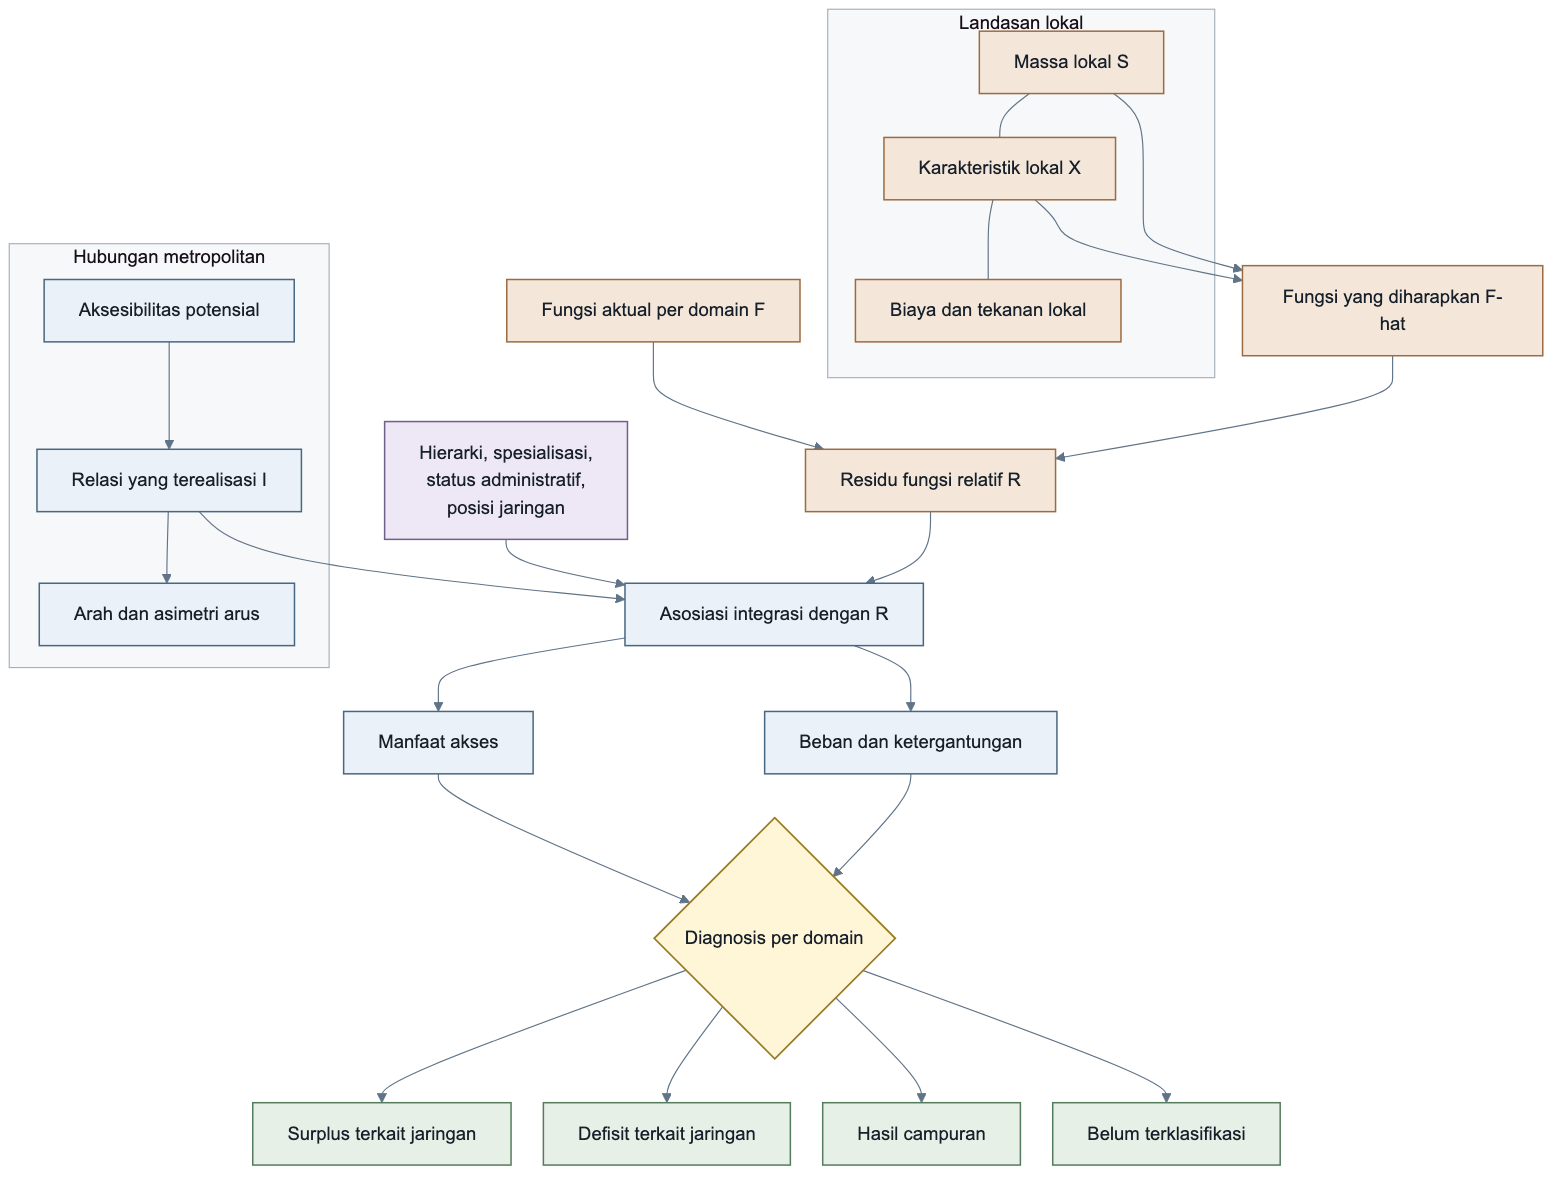
\includegraphics[width=0.88\textwidth]{figures/bab2_kerangka_konseptual.png}
  \caption{Kerangka konseptual hubungan massa lokal, relasi metropolitan, fungsi relatif, manfaat, beban, dan diagnosis per domain. Panah menunjukkan urutan pengukuran dan hubungan yang diuji, bukan hubungan kausal yang telah terbukti.}
  \label{fig:bab2-kerangka-konseptual}
\end{figure}

\subsection{Model pengukuran konseptual}

Untuk setiap pusat $i$ dan domain fungsi $k$, penelitian membedakan:

\begin{enumerate}
  \item ukuran dan karakteristik lokal $(S_i,X_i)$;
  \item integrasi relasional $(I_i)$ yang idealnya berasal dari arus atau interaksi;
  \item fungsi aktual $(F_{ik})$;
  \item fungsi yang diharapkan $(\widehat{F}_{ik})$;
  \item residu fungsi relatif $(R_{ik})$;
  \item manfaat akses $(A_{ik})$;
  \item beban atau ketergantungan $(D_{ik})$; dan
  \item ketahanan klasifikasi $(Q_i)$ berdasarkan variasi spesifikasi yang masih masuk akal.
\end{enumerate}

Hubungan konseptualnya dapat ditulis sebagai:

\[
R_{ik}=g_k(I_i,S_i,X_i,Z_i)+\varepsilon_{ik},
\]

\noindent dengan $Z_i$ sebagai moderator kontekstual. Persamaan ini bukan komitmen pada model kausal. Ia hanya menunjukkan objek yang perlu dipisahkan pada Bab 3: fungsi relatif sebagai keluaran, ukuran dan karakteristik lokal sebagai garis dasar, integrasi sebagai relasi, serta moderator dan ketidakpastian sebagai konteks.

\subsection{Tipologi diagnosis sementara}

\begin{table}[H]
\centering
\caption{Tipologi diagnosis berdasarkan relasi, fungsi relatif, dan beban}
\label{tab:tipologi}
\begin{adjustbox}{max width=\textwidth}
\begin{tabular}{p{0.18\textwidth}p{0.14\textwidth}p{0.18\textwidth}p{0.20\textwidth}p{0.24\textwidth}}
\toprule
\textbf{Integrasi} & \textbf{Residu} & \textbf{Beban} & \textbf{Kelas sementara} & \textbf{Interpretasi aman}\\
\midrule
Tinggi & Positif & Rendah hingga sedang & \textit{Borrowed size} atau integrasi produktif & Pola konsisten dengan akses jaringan yang memperbesar fungsi relatif.\\
Tinggi & Positif & Tinggi & Campuran atau \textit{contested} & Surplus hadir, tetapi manfaat disertai ketergantungan atau beban.\\
Tinggi & Negatif & Tinggi & \textit{Agglomeration shadow} atau ketergantungan asimetris & Integrasi tidak diikuti pematangan fungsi lokal.\\
Tinggi & Negatif & Rendah atau belum terbukti & Terintegrasi tetapi tertinggal & Belum cukup bukti untuk label \textit{shadow}.\\
Rendah & Positif & Bervariasi & Relatif independen atau matang lokal & Surplus tidak terutama dibaca sebagai hasil hubungan dengan Jakarta.\\
Rendah & Negatif & Bervariasi & Periferi lemah & Basis lokal dan hubungan metropolitan sama-sama terbatas.\\
\bottomrule
\end{tabular}
\end{adjustbox}
\end{table}

Kelas akhir dibentuk setelah indikator, arah hubungan, kualitas data, dan sensitivitas diperiksa. Indeks komposit hanya digunakan apabila penggabungan tersebut tidak menyembunyikan perbedaan domain. Jika hasil tidak stabil, unit dilaporkan sebagai berpindah kelas atau belum terklasifikasi.

\subsection{Proposisi empiris}

Proposisi berikut menjadi panduan pengujian, bukan hipotesis kausal yang harus dipaksakan:

\begin{enumerate}
  \item Setelah ukuran dan karakteristik lokal diperhitungkan, integrasi fungsional yang lebih kuat dapat berasosiasi dengan surplus pada sebagian fungsi, tetapi tidak harus pada semua fungsi.
  \item Pada pusat tertentu, integrasi yang kuat dapat berasosiasi dengan defisit fungsi relatif dan beban ketergantungan yang lebih tinggi.
  \item Arah dan besar hubungan dapat berbeda antara pekerjaan, layanan, amenitas, fungsi keputusan, dan kinerja.
  \item Basis lokal, sentralitas, dan kapasitas penyerapan yang lebih kuat dapat membantu pusat mengubah akses jaringan menjadi pematangan fungsi.
  \item Polisentrisitas morfologis tidak dengan sendirinya menjelaskan integrasi fungsional, surplus fungsi, atau rendahnya ketergantungan.
  \item Sebagian unit dapat berpindah kelas ketika proksi, bobot, ambang, atau wilayah tangkapan diubah; unit yang stabil lebih layak menjadi dasar interpretasi.
\end{enumerate}

\subsection{Gerbang penggunaan label}

Label \textit{borrowed size} atau \textit{agglomeration shadow} digunakan hanya jika empat syarat terpenuhi:

\begin{enumerate}
  \item terdapat bukti relasional atau estimasi yang diperiksa terhadap bukti independen;
  \item fungsi aktual dibandingkan dengan ekspektasi ukuran pada unit pembanding yang memadai;
  \item unit, periode, wilayah tangkapan, populasi sasaran, dan konstruk cukup kompatibel; dan
  \item hasil tidak bergantung pada satu proksi lemah atau satu keputusan teknis.
\end{enumerate}

Jika salah satu syarat gagal, istilah yang dipakai adalah aksesibilitas potensial, surplus atau defisit fungsi relatif, ketergantungan komuter, atau pola yang belum terklasifikasi. Aturan ini menjaga agar bahasa teori tidak melampaui status bukti.

\subsection{Posisi penelitian}

Penelitian ini membaca Jabodetabek sebagai sistem metropolitan dengan inti dominan dan sejumlah kandidat pusat sekunder. Relasi antarpusat dapat saling melengkapi, bersaing, atau bergantung. Sumber terbuka dan proksi menjadi dasar pengukuran karena dapat menyediakan lokasi, atribut, jaringan, dan seri waktu yang lebih mudah diulang daripada sumber resmi yang tersedia secara terputus. Keunggulan proksi tetap diuji melalui kesesuaian konstruk, cakupan, keterulangan, biaya, validasi terbuka, dan sensitivitas.

Bab 3 menerjemahkan kerangka ini ke dalam operasionalisasi. Observasi dipisahkan dari agregat, proksi, estimasi, dan simulasi. Periode hanya dibandingkan ketika serinya sebanding. Keluaran yang tidak memenuhi gerbang bukti dilaporkan sebagai diagnosis terbatas. Kerangka teoretis ini tidak menjanjikan panel lengkap atau hubungan kausal yang belum didukung data.

\printbibliography[title={Daftar Pustaka Bab 2}]
\end{document}
